\documentclass[10pt]{beamer}

  % Math Packages
  \usepackage{amsmath}
  \usepackage{amsthm}
  \usepackage{mathtools}

  % Graphics Packages
  \usepackage{graphicx}
  \graphicspath{ {../_static/images/} }
  \usepackage{pgf}
  \usepackage[export]{adjustbox}

  % Code listings
  \usepackage{listings}
  \lstset{language=Python, basicstyle=\footnotesize}

  % Layout
  \usepackage{multicol}

  % Colors
  \definecolor{myblue}{RGB}{25,98,148}
  \definecolor{mygray}{RGB}{66,66,66}

  % Theme Settings
  \usetheme[subsectionpage=progressbar]{metropolis}

  % \setbeamercolor{normal text}{fg=mygray}
  % \setbeamercolor{alerted text}{fg=myblue}
  % \setbeamercolor{title text}{fg=mygray}
  % \setbeamercolor{title separator}{fg=myblue}
  % \setbeamercolor{progress bar}{fg=myblue}
  % \setbeamercolor{frametitle}{bg=myblue}

\title{Writing Python packages}

\date[]{\today}

\begin{document}

% Title Slide
\begin{frame}
  \titlepage
\end{frame}

% ------------------------- %
% Motivation
% ------------------------- %
\section{``Good'' research}

  \begin{frame} \frametitle{What does good research look like?}

    Good research is

    \begin{enumerate}
      \item Accurate: Ensures that what you are doing is what you say you are doing
      \item Collaborative: Working together is better than working alone
      \item Constructive: Engages with work that has been previously done
      \item Foundational: Encourages others to build on your work
    \end{enumerate}

    How can we ensure our research reflects these values?

  \end{frame}

  \begin{frame} \frametitle{Themes of this weekend}

    This weekend we will cover tools that we think help with achieving these values, including,

    \begin{itemize}
      \item Code style, code modularity, and package development
      \item Unit and integration testing
      \item Model testing
    \end{itemize}

  \end{frame}


% ------------------------- %
% Code structure and style
% ------------------------- %
\section{Code structure and style}

  \begin{frame} \frametitle{Stylistic Python code}

    \textbf{Coding is a form of communication\dots}

    \vspace{0.3cm}

    \begin{quote}
      Always code as if the guy who ends up maintaining your code will be a violent psychopath who
      knows where you live. Code for readability. --- Unnamed intelligent coder
    \end{quote}

    \vspace{0.1cm}

    \begin{quote}
      Measuring programming progress by lines of code is like measuring aircraft building progress
      by weight --- Bill Gates
    \end{quote}

  \end{frame}

  \begin{frame} \frametitle{``Non-negotiable'' stylistic rules}

    These are rules I feel (maybe overly) strongly about,

    \begin{itemize}
      \item A space after EVERY comma... Except when trailing --- \texttt{foo = (0,)}
      \item Avoid wildcard imports (i.e. \texttt{from <module> import *})
      \item Four spaces for block indentation... No more, no less.
      \item Limit lines of code to roughly 80 characters
      \item Try to organize code into logical blocks
      \item No space before or after a colon
    \end{itemize}

  \end{frame}

  \begin{frame} \frametitle{Stylistic choices}

    I feel less strongly about some of these rules, but I find that they improve readability for me

    \begin{itemize}
      \item Line breaks should occur before a binary operator
      \item Two lines before and after a function definition
      \item Don't repeat yourself (DRY)
      \item Don't align your \texttt{=}
    \end{itemize}

  \end{frame}

  \begin{frame}[fragile] \frametitle{Examples of good code}

      \begin{lstlisting}{GoodCode}

      import numpy as np
      from scipy.linalg import lstsq


      # Create data
      y = np.array([1.0, 4.0, 3.0, 2.0])
      x = np.array([
          [1.0, 0.5],
          [1.0, 2.0],
          [1.0, 1.5],
          [1.0, 1.0]
      ])

      # Find coefficients
      coeffs, resid, _, _ = lstsq(x, y)

      \end{lstlisting}

  \end{frame}

  \begin{frame}[fragile] \frametitle{Examples of bad code}

      \begin{lstlisting}{BadCode}

      import numpy as np
      from scipy.linalg import *
      y = np.array([1.0, 4.0, 3.0,2.0])
      x = np.array([[1.0,0.5],[1.0,2.0],[1.0, 1.5],[1.0, 1.0]])
      coeffs,resid,_,_ = lstsq(x,y)

      \end{lstlisting}

  \end{frame}



% ------------------------- %
% Exercise
% ------------------------- %
\section{Motivational exercise!}

  \begin{frame} \frametitle{Exercise: Why write packages?}

    We are going to begin by doing some economics for two reasons,

    \begin{enumerate}
      \item We are economists and I'd like us to reflect on how what we learn will be helpful to us
            as economists
      \item Understanding the improvements gained from writing good code/packages has always
            motivated me to strive for high quality code
    \end{enumerate}

  \end{frame}

  \begin{frame} \frametitle{Hendricks Leukhina 2017}

    We start by discussing the paper ``How risky is college investment.''

    \begin{itemize}
      \item One of key components of risk to consider when deciding on college is ``failure to
            graduate'' risk
      \item To motivate the credit accumulation component of their structural model, the authors
            propose a simplified model of credit accumulation
      \item We will replicate certain aspects of this component of their paper (Section 2)
    \end{itemize}

  \end{frame}

  \begin{frame} \frametitle{Exercise instructions}

    Everyone should clone the \texttt{nyupredocs/transcriptestimation} repository found at
    \url{https://www.github.com/nyupredocs}

    You can choose to either work alone or in small (2-3) groups

    Once you have separated into groups, you will be asked to work with one of two versions of the
    replication code. These versions are simply in the \texttt{version\_1} and \texttt{version\_2}
    branches of the repository

    On the next slide, you will be asked to answer some questions using the code provided (and any
    additional code that you will need to write)

  \end{frame}

  \begin{frame} \frametitle{Exercise}

    Do cool stuff

  \end{frame}

  \begin{frame} \frametitle{Debrief}

    How did you find the exercise?

    Which components of code were helpful? What slowed you down?

  \end{frame}



% ------------------------- %
% Package development
% ------------------------- %
\section{Package development}

  \begin{frame} \frametitle{Example package: pyblp}

    \begin{center}
      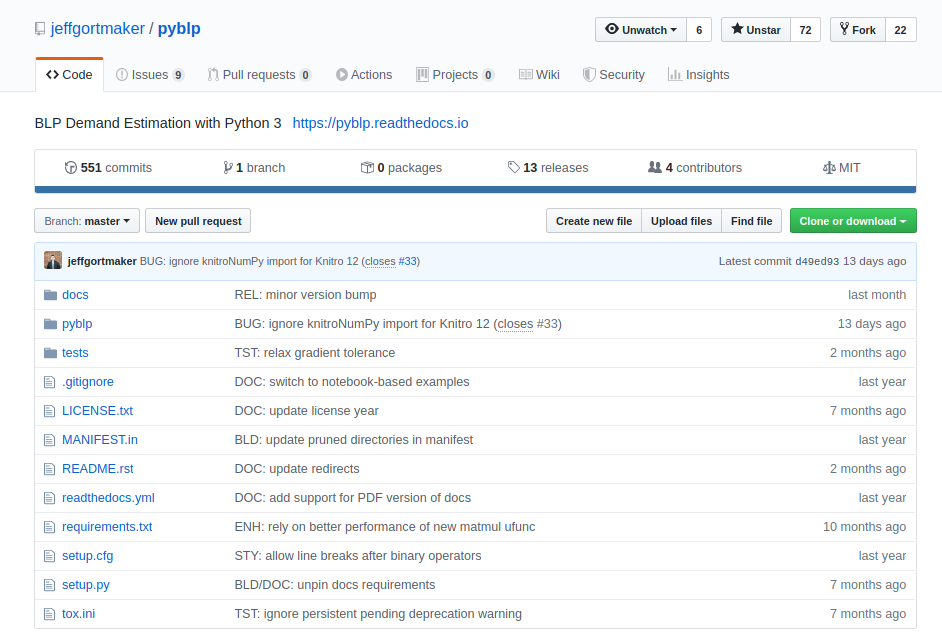
\includegraphics[width=\textwidth]{pyblp_gh_snapshot.png}
    \end{center}

  \end{frame}

  \begin{frame} \frametitle{Package structure}

    {\footnotesize
    Most Python packages share a similar structure

    \begin{itemize}
      \item \texttt{docs}: This folder contains the files that help generate the documentation.
      \item \texttt{<package\_name>}: This folder contains the package source code and is what will
        be loaded by Python when \texttt{import <package\_name} is called.
      \item \texttt{tests}: This folder contains the unit and integration tests
      \item \texttt{README.\{md,rst,txt\}}: This is a file that introduces the package and will be
        rendered on the github landing page.
      \item \texttt{LICENSE.txt}: You should not use a package that is not licensed because
        (according to people who know more about the law than I do) your work is under an
        exclusive copyright by default. Useful to read through \url{https://choosealicense.com}
        to learn a bit more about each license. I tend to prefer relatively permissive Apache/BSD/MIT
        licenses as opposed to copyleft licenses like GPL.
      \item Various files used to build and maintain the package. These files include
        \texttt{setup.py}, \texttt{readthedocs.yml}, \texttt{requirements.txt}, etc\dots
    \end{itemize}

    }

  \end{frame}

  \subsection{Package source code}

  \begin{frame}[fragile] \frametitle{Package source code: structure}

    The package source code is organized into a collection of files and folders. We will
    refer to the folders within the package as ``sub-packages''\footnote{
    Some people get technical and refer to the elements inside of a package as modules,
    sub-modules, and sub-packages, but we're going to try and avoid these details for
    now\dots See
    \href{
    https://stackoverflow.com/questions/7948494/whats-the-difference-between-a-python-module-and-a-python-package
    }{this SO question} if you'd like to know more of the details}.

    In \texttt{pyblp} there is a class called \texttt{SimulationMarket} in
    \texttt{pyblp/markets/simulation\_market.py}. There are two ways to access this class in
    your Python code

    \begin{lstlisting}
    import pyblp

    pyblp.markets.SimulationMarket(args...)
    \end{lstlisting}

    or

    \begin{lstlisting}
    from pyblp.markets import SimulationMarket

    SimulationMarket(args...)
    \end{lstlisting}

  \end{frame}

  \begin{frame} \frametitle{Package source code: \texttt{\_\_init\_\_.py}}

    Your Python package should also have an \texttt{\_\_init\_\_.py} file within the main
    source code directory and within each sub-package.

    \vspace{0.25cm}

    This file used to be required in order to identify a directory as a package, but, as
    of Python 3.3, it is no longer a requirement. However, it is still a good idea to
    include this file because it will be run whenever the package is imported and can be
    a good place to initialize relevant features or expose particular methods.

    \vspace{0.25cm}

    Can find more details in
    \href{http://python-notes.curiousefficiency.org/en/latest/python_concepts/import_traps.html}{this blogpost}

  \end{frame}

  \subsection{Documentation}

  \begin{frame} \frametitle{Documentation: writing docstrings}

    Documentation is your chance to provide your users (including yourself!) instructions
    on what each function does and how it should be used. The vast majority of functions
    should have a doc string.

    \vspace{0.25cm}

    I like to follow the
    \href{https://numpydoc.readthedocs.io/en/latest/format.html}{numpydoc docstring guide},
    but any format you like is fine as long as you're consistent

  \end{frame}

  \begin{frame}[fragile] \frametitle{Documentation: numpydoc docstring conventions}

    \begin{lstlisting}{numpydoc}
    def myfunction(arg1, arg2):
        """
        This paragraph provides a description of the function.

        Parameters
        ----------
        arg1 : type(arg1)
            Description of arg1
        arg2 : type(arg2)
            Description of arg2

        Returns
        -------
        return_value : type(return_value)
            Description of return value

        See Also
        --------
        other_function : This is a related function
        """
        ...
    \end{lstlisting}

  \end{frame}

  \begin{frame}[fragile] \frametitle{Documentation: sphinx}

    \textbf{Step 1}: Create a folder called \texttt{docs}. Within that folder run the
    command \texttt{sphinx-quickstart} from a terminal

    \vspace{0.25cm}

    \textbf{Step 2}: Edit \texttt{conf.py}
    \begin{itemize}
      \item Ensure that the first code in the file includes
        \begin{lstlisting}
        import os
        import sys
        sys.path.insert(0, os.path.abspath(".."))
        \end{lstlisting}
        which ensures that your packages will be found.
      \item Add relevant extensions to \texttt{extensions} variable ---
        This includes at least \texttt{sphinx.ext.autodoc} and
        \texttt{sphinx.ext.napoleon}\footnote{The napoleon extension is required for
        sphinx to understand documentation written according to the numpy or google
        standards. The autodoc extensions is just to simplify your life.}
    \end{itemize}

  \end{frame}

  \begin{frame} \frametitle{Documentation: sphinx}

     \textbf{Step 3}: Generate documentation from your package by running
     \texttt{sphinx-apidoc -o source/  ../<package\_name>} in a terminal in
     the \texttt{docs} directory

     \vspace{0.25cm}

     \textbf{Step 4}: Run \texttt{make html} in a terminal from the \texttt{docs}
     directory

     \vspace{0.25cm}

     \textbf{Step 5}: Open \texttt{\_build/html/index.html} in a browser and review the
     excruciatingly ugly docs generated! Clicking on \textit{Module Index} will take you
     to a page which has the documentation for all of your functions!

  \end{frame}

  \begin{frame} \frametitle{Documentation: sphinx}

    The first step to making the documentation slightly less ugly is to edi the
    \texttt{index.rst} file. It helps to add an introduction to your package at the top
    of the page.

    \vspace{0.25cm}

    You can (and should) also write some instructions for how users could use your
    package.

    \vspace{0.25cm}

    \texttt{pyblp} has an exceptionally good documentation page\dots You should mimic
    the level of detail included.

  \end{frame}

  \begin{frame} \frametitle{Documentation: Read the Docs}

    Read the Docs\footnote{Many of the sites on their page can also be accessed with
    \href{https://www.urbandictionary.com/define.php?term=RTFD}{https://rtfd.org}} is a
    site that hosts documentation (and, more importantly, automates documentation
    updates).

    \vspace{0.25cm}

    Many open source projects use Read the Docs to host their documentation because of
    its ease of use and flexibility

  \end{frame}

  \begin{frame} \frametitle{Documentation: Read the Docs}

    \textbf{Step 1}: Create an account (I find it helpful to use oauth with my github
    account).

    \vspace{0.25cm}

    \textbf{Step 2}: Import your package using their tool --- Doing this takes care of
    webhook that will automatically rebuild your docs whenever a push happens
    to the desired branch

  \end{frame}

  \subsection{Python Package Index}

  \begin{frame} \frametitle{Python Package Index}

    The Python Package Index (PyPI) is ``a repository of software for the Python programming
    language.'' There are over 200,000 projects currently on PyPI

    \vspace{0.3cm}

    Any package on PyPI should be able to be installed with pip\footnote{pip is a recursive
    acronym and stands for \textit{pip installs packages}} by running
    \texttt{pip install <package\_name>}

  \end{frame}


% ------------------------- %
% Package development
% ------------------------- %
\section{Creating your own package}

  \begin{frame} \frametitle{}
  \end{frame}


% --------------------------------- %
% Exercise: Write your own package
% --------------------------------- %
\section{Exercise: Writing your own package}


\end{document}

